\documentclass[tikz]{standalone}
\usepackage{tikz}
\usetikzlibrary{positioning}
\begin{document}
      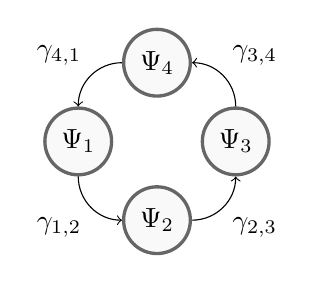
\begin{tikzpicture}[                                                                     
                          bend angle=45,
                          roundnode/.style={                                                   
                                            circle,                                            
                                            draw=black!60,                                     
                                            fill=gray!5,                                       
                                            very thick,                                        
                                            minimum size=7mm                                   
                                           },
                         ]
        \node[roundnode] (top) at (90:1) {$\Psi_{4}$};
        \node[roundnode] (bottom) at (270:1) {$\Psi_{2}$};
        \node[roundnode] (left) at (180:1) {$\Psi_{1}$} 
          edge[<-, bend left] node[auto] {$\gamma_{4,1}$} (top)
          edge[->, bend right] node[auto, swap] {$\gamma_{1,2}$} (bottom); 
        \node[roundnode] (right) at (0:1) {$\Psi_{3}$}
          edge[->, bend right] node[auto, swap] {$\gamma_{3,4}$} (top)
          edge[<-, bend left] node[auto] {$\gamma_{2,3}$} (bottom); 
      \end{tikzpicture}
\end{document}
